
%% bare_jrnl_compsoc.tex
%% V1.4b
%% 2015/08/26
%% by Michael Shell
%% See:
%% http://www.michaelshell.org/
%% for current contact information.
%%
%% This is a skeleton file demonstrating the use of IEEEtran.cls
%% (requires IEEEtran.cls version 1.8b or later) with an IEEE
%% Computer Society journal paper.
%%
%% Support sites:
%% http://www.michaelshell.org/tex/ieeetran/
%% http://www.ctan.org/pkg/ieeetran
%% and
%% http://www.ieee.org/

%%*************************************************************************
%% Legal Notice:
%% This code is offered as-is without any warranty either expressed or
%% implied; without even the implied warranty of MERCHANTABILITY or
%% FITNESS FOR A PARTICULAR PURPOSE! 
%% User assumes all risk.
%% In no event shall the IEEE or any contributor to this code be liable for
%% any damages or losses, including, but not limited to, incidental,
%% consequential, or any other damages, resulting from the use or misuse
%% of any information contained here.
%%
%% All comments are the opinions of their respective authors and are not
%% necessarily endorsed by the IEEE.
%%
%% This work is distributed under the LaTeX Project Public License (LPPL)
%% ( http://www.latex-project.org/ ) version 1.3, and may be freely used,
%% distributed and modified. A copy of the LPPL, version 1.3, is included
%% in the base LaTeX documentation of all distributions of LaTeX released
%% 2003/12/01 or later.
%% Retain all contribution notices and credits.
%% ** Modified files should be clearly indicated as such, including  **
%% ** renaming them and changing author support contact information. **
%%*************************************************************************


% *** Authors should verify (and, if needed, correct) their LaTeX system  ***
% *** with the testflow diagnostic prior to trusting their LaTeX platform ***
% *** with production work. The IEEE's font choices and paper sizes can   ***
% *** trigger bugs that do not appear when using other class files.       ***                          ***
% The testflow support page is at:
% http://www.michaelshell.org/tex/testflow/


\documentclass[10pt,journal,compsoc]{IEEEtran}
%
% If IEEEtran.cls has not been installed into the LaTeX system files,
% manually specify the path to it like:
% \documentclass[10pt,journal,compsoc]{../sty/IEEEtran}





% Some very useful LaTeX packages include:
% (uncomment the ones you want to load)


% *** MISC UTILITY PACKAGES ***
%
%\usepackage{ifpdf}
% Heiko Oberdiek's ifpdf.sty is very useful if you need conditional
% compilation based on whether the output is pdf or dvi.
% usage:
% \ifpdf
%   % pdf code
% \else
%   % dvi code
% \fi
% The latest version of ifpdf.sty can be obtained from:
% http://www.ctan.org/pkg/ifpdf
% Also, note that IEEEtran.cls V1.7 and later provides a builtin
% \ifCLASSINFOpdf conditional that works the same way.
% When switching from latex to pdflatex and vice-versa, the compiler may
% have to be run twice to clear warning/error messages.






% *** CITATION PACKAGES ***
%
\ifCLASSOPTIONcompsoc
  % IEEE Computer Society needs nocompress option
  % requires cite.sty v4.0 or later (November 2003)
  \usepackage[nocompress]{cite}
\else
  % normal IEEE
  \usepackage{cite}
\fi
% cite.sty was written by Donald Arseneau
% V1.6 and later of IEEEtran pre-defines the format of the cite.sty package
% \cite{} output to follow that of the IEEE. Loading the cite package will
% result in citation numbers being automatically sorted and properly
% "compressed/ranged". e.g., [1], [9], [2], [7], [5], [6] without using
% cite.sty will become [1], [2], [5]--[7], [9] using cite.sty. cite.sty's
% \cite will automatically add leading space, if needed. Use cite.sty's
% noadjust option (cite.sty V3.8 and later) if you want to turn this off
% such as if a citation ever needs to be enclosed in parenthesis.
% cite.sty is already installed on most LaTeX systems. Be sure and use
% version 5.0 (2009-03-20) and later if using hyperref.sty.
% The latest version can be obtained at:
% http://www.ctan.org/pkg/cite
% The documentation is contained in the cite.sty file itself.
%
% Note that some packages require special options to format as the Computer
% Society requires. In particular, Computer Society  papers do not use
% compressed citation ranges as is done in typical IEEE papers
% (e.g., [1]-[4]). Instead, they list every citation separately in order
% (e.g., [1], [2], [3], [4]). To get the latter we need to load the cite
% package with the nocompress option which is supported by cite.sty v4.0
% and later. Note also the use of a CLASSOPTION conditional provided by
% IEEEtran.cls V1.7 and later.





% *** GRAPHICS RELATED PACKAGES ***
%
\ifCLASSINFOpdf
  \usepackage[pdftex]{graphicx}
  % declare the path(s) where your graphic files are
  \graphicspath{{./graphics/}}
  % and their extensions so you won't have to specify these with
  % every instance of \includegraphics
  \DeclareGraphicsExtensions{.pdf,.jpeg,.png}
\else
  % or other class option (dvipsone, dvipdf, if not using dvips). graphicx
  % will default to the driver specified in the system graphics.cfg if no
  % driver is specified.
  \usepackage[dvips]{graphicx}
  % declare the path(s) where your graphic files are
  % \graphicspath{{../eps/}}
  % and their extensions so you won't have to specify these with
  % every instance of \includegraphics
  % \DeclareGraphicsExtensions{.eps}
\fi
% graphicx was written by David Carlisle and Sebastian Rahtz. It is
% required if you want graphics, photos, etc. graphicx.sty is already
% installed on most LaTeX systems. The latest version and documentation
% can be obtained at: 
% http://www.ctan.org/pkg/graphicx
% Another good source of documentation is "Using Imported Graphics in
% LaTeX2e" by Keith Reckdahl which can be found at:
% http://www.ctan.org/pkg/epslatex
%
% latex, and pdflatex in dvi mode, support graphics in encapsulated
% postscript (.eps) format. pdflatex in pdf mode supports graphics
% in .pdf, .jpeg, .png and .mps (metapost) formats. Users should ensure
% that all non-photo figures use a vector format (.eps, .pdf, .mps) and
% not a bitmapped formats (.jpeg, .png). The IEEE frowns on bitmapped formats
% which can result in "jaggedy"/blurry rendering of lines and letters as
% well as large increases in file sizes.
%
% You can find documentation about the pdfTeX application at:
% http://www.tug.org/applications/pdftex






% *** MATH PACKAGES ***
%
%\usepackage{amsmath}
% A popular package from the American Mathematical Society that provides
% many useful and powerful commands for dealing with mathematics.
%
% Note that the amsmath package sets \interdisplaylinepenalty to 10000
% thus preventing page breaks from occurring within multiline equations. Use:
%\interdisplaylinepenalty=2500
% after loading amsmath to restore such page breaks as IEEEtran.cls normally
% does. amsmath.sty is already installed on most LaTeX systems. The latest
% version and documentation can be obtained at:
% http://www.ctan.org/pkg/amsmath





% *** SPECIALIZED LIST PACKAGES ***
%
%\usepackage{algorithmic}
% algorithmic.sty was written by Peter Williams and Rogerio Brito.
% This package provides an algorithmic environment fo describing algorithms.
% You can use the algorithmic environment in-text or within a figure
% environment to provide for a floating algorithm. Do NOT use the algorithm
% floating environment provided by algorithm.sty (by the same authors) or
% algorithm2e.sty (by Christophe Fiorio) as the IEEE does not use dedicated
% algorithm float types and packages that provide these will not provide
% correct IEEE style captions. The latest version and documentation of
% algorithmic.sty can be obtained at:
% http://www.ctan.org/pkg/algorithms
% Also of interest may be the (relatively newer and more customizable)
% algorithmicx.sty package by Szasz Janos:
% http://www.ctan.org/pkg/algorithmicx




% *** ALIGNMENT PACKAGES ***
%
\usepackage{array}
% Frank Mittelbach's and David Carlisle's array.sty patches and improves
% the standard LaTeX2e array and tabular environments to provide better
% appearance and additional user controls. As the default LaTeX2e table
% generation code is lacking to the point of almost being broken with
% respect to the quality of the end results, all users are strongly
% advised to use an enhanced (at the very least that provided by array.sty)
% set of table tools. array.sty is already installed on most systems. The
% latest version and documentation can be obtained at:
% http://www.ctan.org/pkg/array


% IEEEtran contains the IEEEeqnarray family of commands that can be used to
% generate multiline equations as well as matrices, tables, etc., of high
% quality.




% *** SUBFIGURE PACKAGES ***
%\ifCLASSOPTIONcompsoc
%  \usepackage[caption=false,font=footnotesize,labelfont=sf,textfont=sf]{subfig}
%\else
%  \usepackage[caption=false,font=footnotesize]{subfig}
%\fi
% subfig.sty, written by Steven Douglas Cochran, is the modern replacement
% for subfigure.sty, the latter of which is no longer maintained and is
% incompatible with some LaTeX packages including fixltx2e. However,
% subfig.sty requires and automatically loads Axel Sommerfeldt's caption.sty
% which will override IEEEtran.cls' handling of captions and this will result
% in non-IEEE style figure/table captions. To prevent this problem, be sure
% and invoke subfig.sty's "caption=false" package option (available since
% subfig.sty version 1.3, 2005/06/28) as this is will preserve IEEEtran.cls
% handling of captions.
% Note that the Computer Society format requires a sans serif font rather
% than the serif font used in traditional IEEE formatting and thus the need
% to invoke different subfig.sty package options depending on whether
% compsoc mode has been enabled.
%
% The latest version and documentation of subfig.sty can be obtained at:
% http://www.ctan.org/pkg/subfig




% *** FLOAT PACKAGES ***
%
%\usepackage{fixltx2e}
% fixltx2e, the successor to the earlier fix2col.sty, was written by
% Frank Mittelbach and David Carlisle. This package corrects a few problems
% in the LaTeX2e kernel, the most notable of which is that in current
% LaTeX2e releases, the ordering of single and double column floats is not
% guaranteed to be preserved. Thus, an unpatched LaTeX2e can allow a
% single column figure to be placed prior to an earlier double column
% figure.
% Be aware that LaTeX2e kernels dated 2015 and later have fixltx2e.sty's
% corrections already built into the system in which case a warning will
% be issued if an attempt is made to load fixltx2e.sty as it is no longer
% needed.
% The latest version and documentation can be found at:
% http://www.ctan.org/pkg/fixltx2e


%\usepackage{stfloats}
% stfloats.sty was written by Sigitas Tolusis. This package gives LaTeX2e
% the ability to do double column floats at the bottom of the page as well
% as the top. (e.g., "\begin{figure*}[!b]" is not normally possible in
% LaTeX2e). It also provides a command:
%\fnbelowfloat
% to enable the placement of footnotes below bottom floats (the standard
% LaTeX2e kernel puts them above bottom floats). This is an invasive package
% which rewrites many portions of the LaTeX2e float routines. It may not work
% with other packages that modify the LaTeX2e float routines. The latest
% version and documentation can be obtained at:
% http://www.ctan.org/pkg/stfloats
% Do not use the stfloats baselinefloat ability as the IEEE does not allow
% \baselineskip to stretch. Authors submitting work to the IEEE should note
% that the IEEE rarely uses double column equations and that authors should try
% to avoid such use. Do not be tempted to use the cuted.sty or midfloat.sty
% packages (also by Sigitas Tolusis) as the IEEE does not format its papers in
% such ways.
% Do not attempt to use stfloats with fixltx2e as they are incompatible.
% Instead, use Morten Hogholm'a dblfloatfix which combines the features
% of both fixltx2e and stfloats:
%
% \usepackage{dblfloatfix}
% The latest version can be found at:
% http://www.ctan.org/pkg/dblfloatfix




%\ifCLASSOPTIONcaptionsoff
%  \usepackage[nomarkers]{endfloat}
% \let\MYoriglatexcaption\caption
% \renewcommand{\caption}[2][\relax]{\MYoriglatexcaption[#2]{#2}}
%\fi
% endfloat.sty was written by James Darrell McCauley, Jeff Goldberg and 
% Axel Sommerfeldt. This package may be useful when used in conjunction with 
% IEEEtran.cls'  captionsoff option. Some IEEE journals/societies require that
% submissions have lists of figures/tables at the end of the paper and that
% figures/tables without any captions are placed on a page by themselves at
% the end of the document. If needed, the draftcls IEEEtran class option or
% \CLASSINPUTbaselinestretch interface can be used to increase the line
% spacing as well. Be sure and use the nomarkers option of endfloat to
% prevent endfloat from "marking" where the figures would have been placed
% in the text. The two hack lines of code above are a slight modification of
% that suggested by in the endfloat docs (section 8.4.1) to ensure that
% the full captions always appear in the list of figures/tables - even if
% the user used the short optional argument of \caption[]{}.
% IEEE papers do not typically make use of \caption[]'s optional argument,
% so this should not be an issue. A similar trick can be used to disable
% captions of packages such as subfig.sty that lack options to turn off
% the subcaptions:
% For subfig.sty:
% \let\MYorigsubfloat\subfloat
% \renewcommand{\subfloat}[2][\relax]{\MYorigsubfloat[]{#2}}
% However, the above trick will not work if both optional arguments of
% the \subfloat command are used. Furthermore, there needs to be a
% description of each subfigure *somewhere* and endfloat does not add
% subfigure captions to its list of figures. Thus, the best approach is to
% avoid the use of subfigure captions (many IEEE journals avoid them anyway)
% and instead reference/explain all the subfigures within the main caption.
% The latest version of endfloat.sty and its documentation can obtained at:
% http://www.ctan.org/pkg/endfloat
%
% The IEEEtran \ifCLASSOPTIONcaptionsoff conditional can also be used
% later in the document, say, to conditionally put the References on a 
% page by themselves.




% *** PDF, URL AND HYPERLINK PACKAGES ***
%
\usepackage{url}
% url.sty was written by Donald Arseneau. It provides better support for
% handling and breaking URLs. url.sty is already installed on most LaTeX
% systems. The latest version and documentation can be obtained at:
% http://www.ctan.org/pkg/url
% Basically, \url{my_url_here}.
\def\UrlBreaks{\do\/\do-}
\usepackage{breakurl}
\usepackage[breaklinks]{hyperref}



% *** Do not adjust lengths that control margins, column widths, etc. ***
% *** Do not use packages that alter fonts (such as pslatex).         ***
% There should be no need to do such things with IEEEtran.cls V1.6 and later.
% (Unless specifically asked to do so by the journal or conference you plan
% to submit to, of course. )


% correct bad hyphenation here
\hyphenation{op-tical net-works semi-conduc-tor}

\usepackage{enumitem,amssymb}
\newlist{todolist}{itemize}{2}
\setlist[todolist]{label=$\square$}
\usepackage{pifont}
\newcommand{\cmark}{\ding{51}}%
\newcommand{\xmark}{\ding{55}}%
\newcommand{\done}{\rlap{$\square$}{\raisebox{2pt}{\large\hspace{1pt}\cmark}}%
	\hspace{-2.5pt}}
\newcommand{\notdone}{\rlap{$\square$}{\large\hspace{1pt}\xmark}}

\usepackage[font=itshape]{quoting}
\usepackage{mdframed}

\mdfdefinestyle{InfoBox}{
	linecolor=black,
	outerlinewidth=2pt,
	%roundcorner=20pt,
	innertopmargin=4pt,
	innerbottommargin=4pt,
	innerrightmargin=4pt,
	innerleftmargin=4pt,
	leftmargin = 4pt,
	rightmargin = 4pt
	backgroundcolor=gray
}

\newtheorem{statement}{Statement}
\usepackage{tabularx}

\begin{document}
%
% paper title
% Titles are generally capitalized except for words such as a, an, and, as,
% at, but, by, for, in, nor, of, on, or, the, to and up, which are usually
% not capitalized unless they are the first or last word of the title.
% Linebreaks \\ can be used within to get better formatting as desired.
% Do not put math or special symbols in the title.
\title{Mobile CI/CD}
%
%
% author names and IEEE memberships
% note positions of commas and nonbreaking spaces ( ~ ) LaTeX will not break
% a structure at a ~ so this keeps an author's name from being broken across
% two lines.
% use \thanks{} to gain access to the first footnote area
% a separate \thanks must be used for each paragraph as LaTeX2e's \thanks
% was not built to handle multiple paragraphs
%
%
%\IEEEcompsocitemizethanks is a special \thanks that produces the bulleted
% lists the Computer Society journals use for "first footnote" author
% affiliations. Use \IEEEcompsocthanksitem which works much like \item
% for each affiliation group. When not in compsoc mode,
% \IEEEcompsocitemizethanks becomes like \thanks and
% \IEEEcompsocthanksitem becomes a line break with idention. This
% facilitates dual compilation, although admittedly the differences in the
% desired content of \author between the different types of papers makes a
% one-size-fits-all approach a daunting prospect. For instance, compsoc 
% journal papers have the author affiliations above the "Manuscript
% received ..."  text while in non-compsoc journals this is reversed. Sigh.

\author{Lukas~Baronyai,~01326526,~lukas.baronyai@tuwien.ac.at}
% \author{Michael~Shell,~\IEEEmembership{Member,~IEEE,}
%         John~Doe,~\IEEEmembership{Fellow,~OSA,}
%         and~Jane~Doe,~\IEEEmembership{Life~Fellow,~IEEE}% <-this % stops a space
% \IEEEcompsocitemizethanks{\IEEEcompsocthanksitem M. Shell was with the Department
% of Electrical and Computer Engineering, Georgia Institute of Technology, Atlanta,
% GA, 30332.\protect\\
% note need leading \protect in front of \\ to get a newline within \thanks as
% \\ is fragile and will error, could use \hfil\break instead.
% E-mail: see http://www.michaelshell.org/contact.html
% \IEEEcompsocthanksitem J. Doe and J. Doe are with Anonymous University.}% <-this % stops an unwanted space
% \thanks{Manuscript received April 19, 2005; revised August 26, 2015.}}

% note the % following the last \IEEEmembership and also \thanks - 
% these prevent an unwanted space from occurring between the last author name
% and the end of the author line. i.e., if you had this:
% 
% \author{....lastname \thanks{...} \thanks{...} }
%                     ^------------^------------^----Do not want these spaces!
%
% a space would be appended to the last name and could cause every name on that
% line to be shifted left slightly. This is one of those "LaTeX things". For
% instance, "\textbf{A} \textbf{B}" will typeset as "A B" not "AB". To get
% "AB" then you have to do: "\textbf{A}\textbf{B}"
% \thanks is no different in this regard, so shield the last } of each \thanks
% that ends a line with a % and do not let a space in before the next \thanks.
% Spaces after \IEEEmembership other than the last one are OK (and needed) as
% you are supposed to have spaces between the names. For what it is worth,
% this is a minor point as most people would not even notice if the said evil
% space somehow managed to creep in.



% The paper headers
% \markboth{Journal of \LaTeX\ Class Files,~Vol.~14, No.~8, August~2015}%
% {Shell \MakeLowercase{\textit{et al.}}: Bare Demo of IEEEtran.cls for Computer Society Journals}
% The only time the second header will appear is for the odd numbered pages
% after the title page when using the twoside option.
% 
% *** Note that you probably will NOT want to include the author's ***
% *** name in the headers of peer review papers.                   ***
% You can use \ifCLASSOPTIONpeerreview for conditional compilation here if
% you desire.



% The publisher's ID mark at the bottom of the page is less important with
% Computer Society journal papers as those publications place the marks
% outside of the main text columns and, therefore, unlike regular IEEE
% journals, the available text space is not reduced by their presence.
% If you want to put a publisher's ID mark on the page you can do it like
% this:
%\IEEEpubid{0000--0000/00\$00.00~\copyright~2015 IEEE}
% or like this to get the Computer Society new two part style.
%\IEEEpubid{\makebox[\columnwidth]{\hfill 0000--0000/00/\$00.00~\copyright~2015 IEEE}%
%\hspace{\columnsep}\makebox[\columnwidth]{Published by the IEEE Computer Society\hfill}}
% Remember, if you use this you must call \IEEEpubidadjcol in the second
% column for its text to clear the IEEEpubid mark (Computer Society jorunal
% papers don't need this extra clearance.)



% use for special paper notices
%\IEEEspecialpapernotice{(Invited Paper)}



% for Computer Society papers, we must declare the abstract and index terms
% PRIOR to the title within the \IEEEtitleabstractindextext IEEEtran
% command as these need to go into the title area created by \maketitle.
% As a general rule, do not put math, special symbols or citations
% in the abstract or keywords.
\IEEEtitleabstractindextext{%
\begin{abstract}
How does an ideal CI/CD pipeline in the mobile (Android) world look like, what are existing best practises, what are possible organisationalen impacts
\end{abstract}

% Note that keywords are not normally used for peerreview papers.
\begin{IEEEkeywords}
Mobile Continuous Integration, Mobile Continuous Delivery, Android.
\end{IEEEkeywords}}


% make the title area
\maketitle


% To allow for easy dual compilation without having to reenter the
% abstract/keywords data, the \IEEEtitleabstractindextext text will
% not be used in maketitle, but will appear (i.e., to be "transported")
% here as \IEEEdisplaynontitleabstractindextext when the compsoc 
% or transmag modes are not selected <OR> if conference mode is selected 
% - because all conference papers position the abstract like regular
% papers do.
\IEEEdisplaynontitleabstractindextext
% \IEEEdisplaynontitleabstractindextext has no effect when using
% compsoc or transmag under a non-conference mode.



% For peer review papers, you can put extra information on the cover
% page as needed:
% \ifCLASSOPTIONpeerreview
% \begin{center} \bfseries EDICS Category: 3-BBND \end{center}
% \fi
%
% For peerreview papers, this IEEEtran command inserts a page break and
% creates the second title. It will be ignored for other modes.
\IEEEpeerreviewmaketitle

\IEEEraisesectionheading{\section{Introduction}\label{sec:introduction}}

CI/CD is a known and well-used process for a majority of software projects - but not yet in the mobile world. In this paper we will take a closer look how CI/CD differs from the "classical" CI/CD definition. The mobile world is heavily dominated by the two major OS Android and iOS - both having their own CI/CD approaches. This paper will only cover the Android way and which official recommendations Google gives. For Apple sources we recommend the official Apple resources as a starting point into the topic.
\footnote{\url{https://developer.apple.com/library/archive/documentation/IDEs/Conceptual/xcode_guide-continuous_integration/}}.

This paper will then apply the gather information in a case study of a mobile software development, developing a prototype pipeline together with a workflow ready to use. The final Bitrise configuration utilizing this process can be found in the Appendix~\ref{bitrise_config}.
\section{Classical CI/CD}

\begin{figure}[htb]
	\centering
	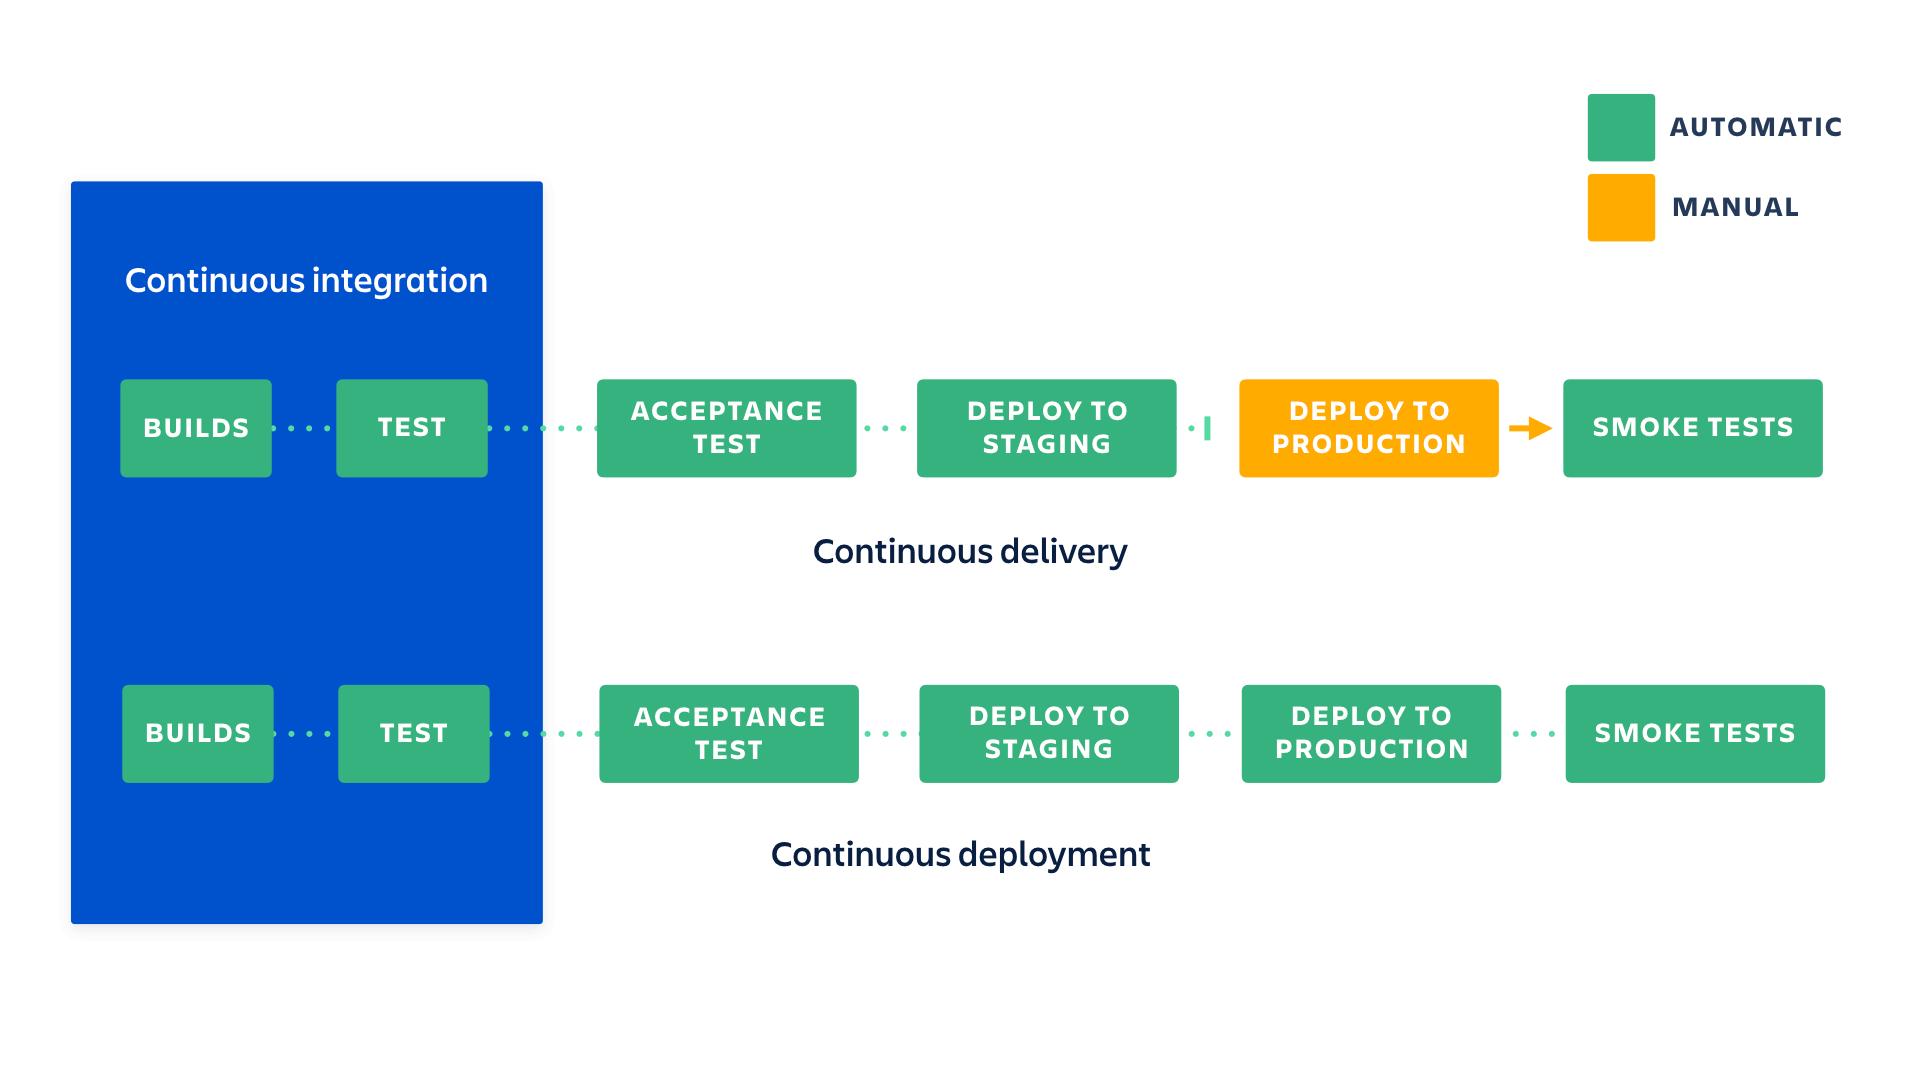
\includegraphics[width=0.5\textwidth]{./ci_cd_cd.png}
	\caption[CI \& CD]{CI \& CD\footnotemark}
	\label{fig_ci_cd}
\end{figure}
\footnotetext{\url{https://wac-cdn.atlassian.com/dam/jcr:b2a6d1a7-1a60-4c77-aa30-f3eb675d6ad6/ci\%20cd\%20asset\%20updates\%20.007.png?cdnVersion=508}}

In order to look into mobile approaches to CI/CD, it is first necessary to have a quick look into the "classical" theory. The original concept was heavily shaped by Kent Beck and Ron Jeffries in the context of their concept of Extreme Programming~\cite{beck1998extreme, beck2000extreme}

\subsection{Continuous Integration}
In his text about Continuous Integration Martin Fowler defined it as follows:

\begin{quoting}
"A software development practice where members of a team integrate their work frequently, usually each person integrates at least daily - leading to multiple integration per day. Each integration is verified by an automated build (including test) to detect integration errors as quickly as possible."~\cite{fowler2006continuous}
\end{quoting}

According to this, the typical workflow in a CI setup looks like the following. During the whole process there is always a high emphasis on monitoring the code state, checking (and preventing) broken code as often as possible. This process replaced the formerly used first-implement-then-integrate approach by integrating the code on a regular (daily) base.

\begin{itemize}
	\item Checkout master branch of repository
	\item Create working copy
	\item Add changes
	\item Check local build
	\item Verify integrity with local tests
	\item Downmerge with master branch
	\item Upmerge with master branch
	\item Automated build at server
	\item Automated testing at server
\end{itemize} 

Additional to this, he gave in the same text 9 practices to use CI. This list will be used in the following as a tool to analyze existing practices and especially to apply it for mobile CI/CD. 

\begin{enumerate}
	\item Maintain a Single Source Repository
	\item Automate the Build
	\item Make Your Build Self-Testing\footnote{\url{https://martinfowler.com/bliki/SelfTestingCode.html}}
	\item Everyone Commits Every Day
	\item Every Commit Should Build the Mainline on an Integration Machine
	\item Keep the Build Fast
	\item Test in a Clone of the Production Environment
	\item Make it Easy for Anyone to Get the Latest Executable
	\item Everyone can see what's happening
\end{enumerate}

\subsection{Continuous Delivery}

Coming from CI, Continuous Delivery builds upon this and adds additionally a manual deployment step to the production environment. So after every test runs through positively, the setup is ready to deploy by a click on a button at any time. But it still has a final human instance in between the push to the repository and the release.

\subsection{Continuous Deployment}

Removing the last human component in this process then leads to Continuous Deployment, making the full process fully automated. Each push the the master branch then automatically leads to a release deployment if the whole pipeline does not detect any failed tests or broken builds.

Disregarding if the last step is now fully automated or only partially with a final human component, I extend the mentioned checklist with:

\begin{enumerate}
	\item[10)] Automate Deployment
\end{enumerate}

\section{Mobile CI/CD}

Coming now from the "classical" CI/CD approach, it is not possible to instantly apply the known model to the mobile world, it needs some adoption. Before we do so, we have to consider the following points: \\

\begin{itemize}
	
	\item \textbf{Mobile application have a high UI focus} \\
	UI tests are always more expensive to create than for "standard" code - and this is even more valid for mobile applications. Additionally from the known challenges of desktop applications like clickable fields, listener states, dependencies between views \& co, a mobile device introduces complexity
	\\
	
	\item \textbf{Mobile applications have per default a build tool} \\
	Both iOS (\textit{XCode}) and Android (\textit{AndroidStudio} \& \textit{gradle}) come along with their own build system and IDE, making the question if the application is build manually or automated with a tool pointless.
	\\
	
	\item \textbf{There is no standard production environment} \\
	Due to the nature of the mobile device world, there is no standard device towards a deployment can happen. Especially but not only with Android there is a huge variety of screen sizes and operating system versions to be handled. Therefore automated testing has to be a compromise between covered variations and invested efforts. There are of course attempts to test with assuming the maximum coverage of variations, but it can never be sufficient as for e.g. a server software.
	\\
	
	\item \textbf{Emulation is expensive} \\
	Another consequence of the variety of device types, testing with real hardware is a pain and lead to the usage of emulators. But emulation is expensive in terms of time and resources, especially since due to the high share of required UI tests, a majority of testing can not be done independent from the (emulated) mobile OS.
	
\end{itemize}

\subsection{Adopted CI/CD model}
As consequence to the mentioned points, we will adopt the practise checklist of Fowler by completely removing 2) (inherited to the build tools) and changing 7) to "Test in a Emulated Environment".

\subsection{Googles CI/CD tools}

Google provides many frameworks and guidelines which can be pretty overwhelming - this and the next section is therefore dedicated to give an overview of these and summarize which options there are to implement a proper CI/CD pipeline within the Android world. 

\subsubsection{Android Emulator}

Bundled within the Android SDK comes the Android Emulator\footnote{\url{https://developer.android.com/studio/run/emulator}}, which allows the emulation of a virtual device on the local machine. It supports various images, called Android Virtual Devices (AVD), with different configuration options. Once launched it is considered as a real device by \texttt{adb} and can therefore used as deployment target. The tool further provides the option to launch without an UI and to be used for testing on a server.

\subsubsection{Firebase Test Lab}
With Firebase Test Lab\footnote{\url{https://firebase.google.com/docs/test-lab/android/overview}} Google offers a cloud-based device farm with virtual and real devices. It supports two different testing methods: Instrumentation (see section~\ref{sec:test_types}) and Robo (basic test type that simulates real user interactions) Tests. Test results are provided with additional logs, videos and screenshots.
Firebase Test Lab allows 10 tests per day for virtual devices and 5 for physical devices in it's free version ("Spark Plan") - but some CI/CD cloud services like Bitrise included the service within their contingents.

\subsubsection{Google Play Deploy}
Google offers via the Play Store console a REST API to deploy compiled APKs and AABs which can be used in an CD setup. The API is secured via the according Service account. Additionally to the (not prefered way) direct release track it is possible to deploy to the \texttt{alpha}, \texttt{beta} or \texttt{internal} tracks\footnote{\url{https://developers.google.com/android-publisher/tracks}}.

\subsubsection{Available CI/CD Server}

In order to properly utilize a mobile CI/CD pipeline there are many estabilshed server provider around - since it would exceed the scope of this paper to make a full comparison of these service providers, we limit it to a selection of the most commons:

\begin{itemize}
	\item Bitrise\footnote{\url{https://www.bitrise.io/}}
	\item TeamCity\footnote{\url{https://www.jetbrains.com/teamcity/}}
	\item Travis CI\footnote{\url{https://travis-ci.org/}}
	\item Jenkins\footnote{\url{https://jenkins.io/}}
	\item Bamboo\footnote{\url{https://www.atlassian.com/software/bamboo}}
	\item GitLab CI/CD\footnote{\url{https://about.gitlab.com/product/continuous-integration/}}
	\item CircleCI\footnote{\url{https://circleci.com/}}
\end{itemize}

\subsection{Android testing}
One of the most crucial steps within a CI/CD pipeline is the testing part. Again, there a many tools around for testing different levels of abstractions and granularity - this paper will foremost focus on the recommended toolchain by the Android project.~\cite{doc:fundamental_testing}

Similar to existing best practices in the "classical" software world, there is a test-driven-development approach, but adopted for a mobile approach. As can be seen in figute~\ref{fig_google_testing} there are two cycles: unit and UI. Since UI testing usually consumes far more time than unit testing, these two are seperated from each other.

\begin{figure}[h]
	\centering
	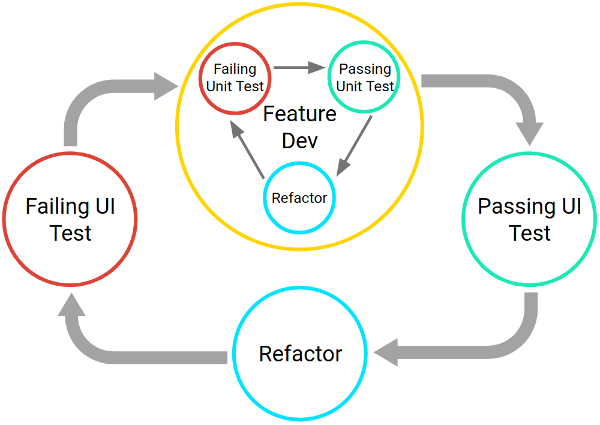
\includegraphics[width=0.5\textwidth]{./google_testing.png}
	\caption[The two cycles associated with iterative, test-driven development]{The two cycles associated with iterative, test-driven development\footnotemark}
	\label{fig_google_testing}
\end{figure}
\footnotetext{\url{https://developer.android.com/images/training/testing/testing-workflow.png}}

Google also defines three types of test categories: (see figure~\ref{fig_google_pyramid})

\begin{figure}[htb]
	\centering
	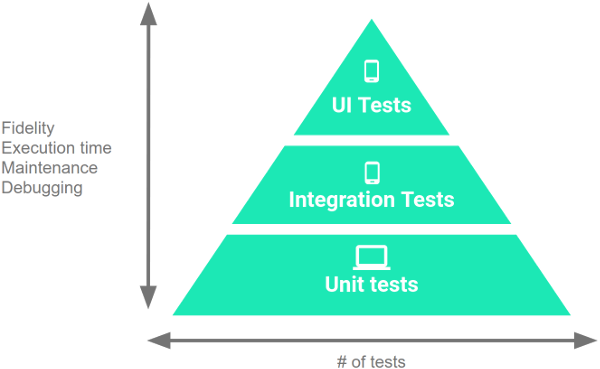
\includegraphics[width=0.5\textwidth]{./pyramid.png}
	\caption[The Testing Pyramid, showing the three categories of tests that should be included in an app's test suite]{The Testing Pyramid, showing the three categories of tests that should be included in an app's test suite\footnotemark}
	\label{fig_google_pyramid}
\end{figure}
\footnotetext{\url{https://developer.android.com/images/training/testing/pyramid.png}}

\begin{itemize}
	\item \textbf{Unit tests - Small tests} \\ 
	These kind of tests validate the behavior of a feature on an atomic level and are highly focues. Around 70\% of the test base should consist of small test, typical frameworks are JUnit, Mockito and PowerMock.
	
	\item \textbf{Integration tests - Medium tests} \\ 
	The next level of testing are the medium/integration tests which are testing the integration of either different level of the the stack within a module or of different modules. The recommendation is to have around 20\% of tests for integration, the toolchain provides Robolectric for this.
	
	\item \textbf{UI tests - Large tests} \\ 
	On top of the testing setup are the large tests, the UI tests. They are used to test end-to-end flows including the interaction of the user with the app through multiple stack level and modules. UI tests are usually very long running flows which have a high ressource impact. It is recommended to have 10\% UI Test, Google provides Espresso and UI Automator on the tool side.
\end{itemize}

For a more detailed overview of the different test size see~\ref{fig_google_test_sizes}.

\begin{figure}[htb]
	\centering
	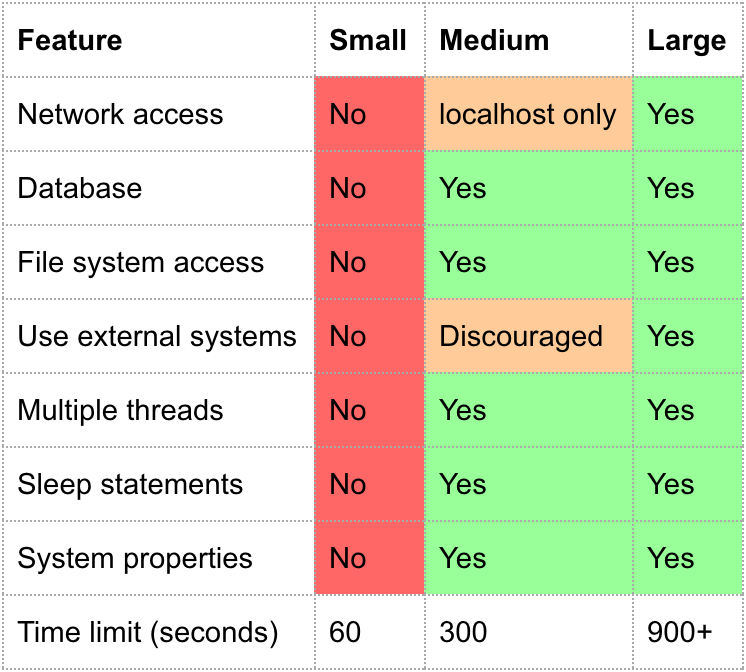
\includegraphics[width=0.5\textwidth]{./test_sizes.png}
	\caption[Test Sizes]{Test Sizes\footnotemark}
	\label{fig_google_test_sizes}
\end{figure}
\footnotetext{\url{https://testing.googleblog.com/2010/12/test-sizes.html}}

Additional to the different test types and sizes, there are also two types of tests based on the environment where they have to be executed:

\begin{itemize}
	\item Normal \textbf{tests}\\
	are executed by the local machine and the JVM and do not require any dependencies to the Android OS. Test resources are located under \texttt{test}.
	\item \textbf{Instrumentation test} \\
	need for execution a mobile device and have a dependency to the Android OS. This device can be physical, virtual (by the Emulator) or simulated (by Roboelectric). Test resources are located under \texttt{androidTest}.
\end{itemize}

Based on this overview of testing classification, the following subsections will give an overview of the tools provided by Google to cover those different levels:

\subsubsection{JUnit, Mockito \& AndroidJUnit4}
The standard JUnit\footnote{\url{https://junit.org/junit4/}} framework is the most obvious solution to build unit tests and is together with Mockito available for use in Android (with JUnit version 4). It is possible to access Android resources within an unit test by configuring gradle with \texttt{unitTests.includeAndroidResources}.

It is further possible to write instrumented JUnit tests by using the \textbf{\texttt{AndroidJUnit4}} test runner (on which e.g. Espresso and UIAutomator relay on). In order to isolate the execution of these tests and to minimize possible shared states between those runs, there is the Android Test Orchestrator\footnote{\url{https://developer.android.com/training/testing/junit-runner}} available.

\subsubsection{Robolectric}
Robolectric\footnote{\url{http://robolectric.org/}} is a framework for unit and integration testing without relaying on a emulator or physical device - instead it uses a simulated device by wrapping the Android framework. This way it can provide far more faster test executions than with instrumentation tests.

\subsubsection{Espresso}
Espresso\footnote{\url{https://developer.android.com/training/testing/espresso}} provides instrumented UI tests with a relatively simple API to use. Next to standard situation with handling UI components, it is able to handle WebViews, idling resources, intents and even multi processes.
Bundled with the \textit{AndroidStudio} comes also the \textbf{Espresso Test Recorder} which simplifies the automatic creation by a great extend - by simply recording an use case.

\subsubsection{UI Automator}
The UI Automator\footnote{\url{https://developer.android.com/training/testing/ui-automator}} framework provides functionality for cross-app UI testing, including interaction between user apps and system apps (e.g. opening the setting menu or app launcher). It further lets tests access hardware functionality such as pressing the Back, Home or Menu buttons or using the volume buttons.

\subsubsection{Android Jetpack Test}

At the I/O18 it the new Android Jetpack component "Android Test"\footnote{\url{https://developer.android.com/training/testing/}} was announced, which aims at unifying the different tools and framework together in one center API within the \textit{AndroidX} package.
At the time of writting this paper, the following tools are fully integrated: Espresso, UI Automator and AndroidJUnitRunner. Robolectric got a major update (v4) for the integration with AndroidX, but is no finished yet.

\begin{mdframed}[style=InfoBox,align=center]
	\textbf{Note:} Google recently (I/O18) also announced "Project Nitrogen" which intents to remove any restrictions of tests to runtime environment - but there are no further information available at the time of writing this paper.
\end{mdframed}

\subsubsection{Outside of the Google ecosystem}

Of course there are many more testing frameworks and tools out there which are not in a direct relation to Google and are not in the standard toolchain. Some well-known examples are:

\begin{itemize}
	\item Appium\footnote{\url{http://appium.io/}}
	\item Detox\footnote{\url{https://github.com/wix/detox}}
	\item Calabash\footnote{\url{http://calaba.sh/}}
	\item screenshot-tests-for-android\footnote{\url{https://facebook.github.io/screenshot-tests-for-android/}}
\end{itemize}




\section{Mobile CI prototype}

\begin{mdframed}[style=InfoBox,align=center]
	\textbf{Note:} Due to the big differences in tools and languages, this paper will only focus on Android CI/CDs. Most of the principles can be used for iOS as well, but the tools will most likely differ
\end{mdframed}

\subsection{About Test Driven Development in the mobile world}
\section{Mobile CI/CD example: AllAboutApps pipeline}
After looking into what options there are to define a CI/CD pipeline for mobile applications, this section will now evaluate this with an existing pipeline at AllAboutApps, how a concrete implementation looks like and how it can be improved to fully apply as CI/CD pipeline.

\subsection{Current state}
The current setup is based on Bitrise and an automated Google Play Store deployment. The current workflow/pipeline looks as follows:\\

\begin{itemize}
	\item Checkout \texttt{master} branch
	\item Create \texttt{feature} branch
	\item Implement feature, commit as atomic as possible
	\item Local builds
	\item Bitrise trigger for push: \texttt{debug} build
	\item If feature fulfills internal \textit{Definition of Done}: pull request
	\item After pull request approval: merge to \texttt{master}
	\item Bitrise trigger for \texttt{master}: release \& preview build
	\item If everything successful: upload to \texttt{internal} or \texttt{alpha} track of Google Play
	\item QA is testing last master build
	\item After QA \& customer approval: promotion to \texttt{release} track in Google Play\\
\end{itemize}

As we can see, this workflow already covers most of the CI/CD steps, but misses some crucial points. In order to analyze how this can be improved to a fully implemented CI/CD pipeline, we will use the previously introduced adopted checklist of Fowler:\\

\begin{enumerate}\label{analysis_aaa}
	
	\item \textbf{Maintain a Single Source Repository}
	\begin{todolist}
		\item[\done] \texttt{Git} is common practice at the company \\
	\end{todolist}

	\item \textbf{Make Your Build Self-Testing}
	\begin{todolist}
		\item[\notdone] No automated testing
		\item[\notdone] No testing culture
		\item Bitrise would support it \\
	\end{todolist}

	\item \textbf{Everyone Commits Every Day}
	\begin{todolist}
		\item[\done] Common practice at the company \\
	\end{todolist}

	\item \textbf{Every Commit Should Build the Mainline on an Integration Machine}
	\begin{todolist}
		\item[\done] Yes by Bitrise push triggers\\
	\end{todolist}

	\item \textbf{Keep the Build Fast}
	\begin{todolist}
		\item[\done] Inherited due to the \texttt{Gradle} build system for Android \\
	\end{todolist}

	\item \textbf{Test in an Emulated Environment}
	\begin{todolist}
		\item[\notdone] No automated testing
		\item Bitrise would support it (all of UI, integration and unit testing) \\
	\end{todolist}

	\item \textbf{Make it Easy for Anyone to Get the Latest Executable}
	\begin{todolist}
		\item[\done] Yes, by Bitrise build artifacts \\
	\end{todolist}

	\item \textbf{Everyone can see what's happening}
	\begin{todolist}
		\item[\done] Covered by Bitrise - everyone has access to the current build states of the projects \\
	\end{todolist}

	\item \textbf{Automate Deployment}
	\begin{todolist}
		\item[\done] Yes, automated deployment to Google Play \texttt{internal} or \texttt{alpha} track, manual deployment to \texttt{release}
	\end{todolist}

\end{enumerate}

\subsection{Missing steps}
As it can be seen in listening~\ref{analysis_aaa}, the biggest issue is that there is currently \textbf{no automated testing} in the existing pipeline. Additionally a requirement analysis pointed out that next to testing there should be a \textbf{static code analysis} (\texttt{kklint}) introduced in the pipeline.

In order to fix this, the company developed a prototype pipeline for an existing project which covers all necessary steps of a full functional CI/CD pipeline. In order to do so, it was necessary to define limitations and a set of statements:\\

\begin{statement}\label{stat:long_ui}
	UI tests are very long running workflows on Bitrise
\end{statement}

\begin{statement}\label{stat:short_unit}
	Unit tests are relatively short running workflows on Bitrise
\end{statement}

\begin{statement}
	Concurrent builds are limited by 3 due to the Bitrise billing limits.
\end{statement}

\begin{statement}
	Pull requests only have 1 trigger at Bitrise, there is (currently) no trigger when updating a pull requests.
\end{statement}

\begin{statement}
	Bitrise includes Firebase Test Lab runs, which are only limited by the maximal build duration.
\end{statement}

\begin{statement}\label{stat:break_builds}
	Changing the pipeline of an existing project towards a full CI/CD pipeline shall not break the existing build without adding failing tests.
\end{statement}

\begin{statement}
	Bitrise supports triggered and scheduled builds.
\end{statement}

\begin{statement}
	The major advantage of Bitrise is the huge supply of Build Step Plugins.\footnote{\url{https://github.com/bitrise-io/bitrise-steplib}}
\end{statement}

\begin{statement}
	Android builds are done with several build variants. (debug/release, production/staging, etc).
\end{statement}

\begin{statement}
	UI requirements are usually changing very fast in projects.
\end{statement}

\subsection{Updated CI/CD pipeline}

\begin{table}[htb]
	\renewcommand{\arraystretch}{1.3}
	\caption{Workflow overview}
	\label{tab:overview_workflows}
	\centering
	\begin{tabular}{|p{31pt}||p{45pt}|p{50pt}|p{45pt}|p{45pt}|}
		\hline
		\textbf{Workflow} & \textbf{\texttt{debug}} & \textbf{\texttt{integration}} & \textbf{\texttt{release}} & \textbf{\texttt{preview}} \\ \hline \hline
		\textbf{Trigger} & push to feature & scheduled daily & tag on master & push to master \& pull requests \\ \hline
		\textbf{Duration} & $\sim$15min & $>$ 1h & $>$ 1h & $\sim$20min \\ \hline
		\textbf{Testtype} & unit \& klint & integration \& UI & full test suite & unit \& klint \\ \hline
		\textbf{Build Variant} & debug & debug & release & preview \\ \hline
		\textbf{Post build} & - & - & Upload to Google Play \texttt{internal}/ \texttt{alpha} track & - \\ \hline
	\end{tabular}
\end{table}

From the conclusion of these statements, there were these workflows defined:

\begin{enumerate}
	\item \textbf{\texttt{debug}}\\
	Runs on every push on feature branches and triggers only unit tests and klint checks. Due to statement~\ref{stat:break_builds} the klint checks per default are configured to not fail the build on reporting errors.
	\item \textbf{\texttt{integration}}\\
	Can only run each nights (using Bitrise's scheduling feature) due to its very long build duration (can even be over an hour). It uses Firebase Robo \& UI testing, Espresso and Robolectrics.
	\item \textbf{\texttt{release}}\\
	Triggered by a \texttt{git tag} and runs each available test suite, including unit, integration and UI tests, before building a release build and uploading it automated to the Google Play \texttt{internal}/\texttt{alpha} track. The final release is done manually.
	\item \textbf{\texttt{preview}}\\
	On each pull request to the master branch and each push to the master itself the \texttt{preview} workflow is triggered, running all unit tests and klint checks.
\end{enumerate}

The full configuration file of Bitrise is referred in the appendix~\ref{bitrise_config}

\subsubsection{Additional remarks \& recommendations}
Due to the nature of the company being an agency instead of doing product development, the outlined CI/CD pipeline is far less sophisticated than it could be. Projects in these kind of companies will never be long term enough to build up big test suites and investing resources into setting up big test cases are always in discrepancy with the project scope. 

But there is always room for improvements, so here are some additional recommendations, how the pipeline could be enhanced:

\begin{itemize}
	\item \textbf{Enhanced Pull Requests}\\
	The current state of pull requests reviews could be enhanced by providing the existing \texttt{klint}/\texttt{detekt} \textbf{reports} together with some other meta information (e.g. changed permission set, increased apk size) in order to make proper use of the existing information and utilize a more informed decision about the pull request.\\
	Further it would make sense to \textbf{analyze commits after opening pull requests} (which Bitrise currently does not support) in order to see the improvements in between these commits.
	\item \textbf{Pre-commit git hooks}\\
	Another quite useful tool are the \texttt{git hooks} which can be run on pre-commit (or pre-push) to trigger e.g. a lint analyses in order to already prevent faulty code in the repository. These hooks could block a push if the committed code does not reach a certain quality goal. And since \texttt{lint}/\texttt{detekt} are usually rather fast tools (which don't even require a full build to run), it would have not a big impact on the development process.
\end{itemize}


\section{Summary}
The summary goes here.


% An example of a floating figure using the icx package.
% Note that \label must occur AFTER (or within) \caption.
% For figures, \caption should occur after the \includegraphics.
% Note that IEEEtran v1.7 and later has special internal code that
% is designed to preserve the operation of \label within \caption
% even when the captionsoff option is in effect. However, because
% of issues like this, it may be the safest practice to put all your
% \label just after \caption rather than within \caption{}.
%
% Reminder: the "draftcls" or "draftclsnofoot", not "draft", class
% option should be used if it is desired that the figures are to be
% displayed while in draft mode.
%
%\begin{figure}[!t]
%\centering
%\includegraphics[width=2.5in]{myfigure}
% where an .eps filename suffix will be assumed under latex, 
% and a .pdf suffix will be assumed for pdflatex; or what has been declared
% via \DeclareGraphicsExtensions.
%\caption{Simulation results for the network.}
%\label{fig_sim}
%\end{figure}

% Note that the IEEE typically puts floats only at the top, even when this
% results in a large percentage of a column being occupied by floats.
% However, the Computer Society has been known to put floats at the bottom.


% An example of a double column floating figure using two subfigures.
% (The subfig.sty package must be loaded for this to work.)
% The subfigure \label commands are set within each subfloat command,
% and the \label for the overall figure must come after \caption.
% \hfil is used as a separator to get equal spacing.
% Watch out that the combined width of all the subfigures on a 
% line do not exceed the text width or a line break will occur.
%
%\begin{figure*}[!t]
%\centering
%\subfloat[Case I]{\includegraphics[width=2.5in]{box}%
%\label{fig_first_case}}
%\hfil
%\subfloat[Case II]{\includegraphics[width=2.5in]{box}%
%\label{fig_second_case}}
%\caption{Simulation results for the network.}
%\label{fig_sim}
%\end{figure*}
%
% Note that often IEEE papers with subfigures do not employ subfigure
% captions (using the optional argument to \subfloat[]), but instead will
% reference/describe all of them (a), (b), etc., within the main caption.
% Be aware that for subfig.sty to generate the (a), (b), etc., subfigure
% labels, the optional argument to \subfloat must be present. If a
% subcaption is not desired, just leave its contents blank,
% e.g., \subfloat[].


% An example of a floating table. Note that, for IEEE style tables, the
% \caption command should come BEFORE the table and, given that table
% captions serve much like titles, are usually capitalized except for words
% such as a, an, and, as, at, but, by, for, in, nor, of, on, or, the, to
% and up, which are usually not capitalized unless they are the first or
% last word of the caption. Table text will default to \footnotesize as
% the IEEE normally uses this smaller font for tables.
% The \label must come after \caption as always.
%
%\begin{table}[!t]
%% increase table row spacing, adjust to taste
%\renewcommand{\arraystretch}{1.3}
% if using array.sty, it might be a good idea to tweak the value of
% \extrarowheight as needed to properly center the text within the cells
%\caption{An Example of a Table}
%\label{table_example}
%\centering
%% Some packages, such as MDW tools, offer better commands for making tables
%% than the plain LaTeX2e tabular which is used here.
%\begin{tabular}{|c||c|}
%\hline
%One & Two\\
%\hline
%Three & Four\\
%\hline
%\end{tabular}
%\end{table}


% Note that the IEEE does not put floats in the very first column
% - or typically anywhere on the first page for that matter. Also,
% in-text middle ("here") positioning is typically not used, but it
% is allowed and encouraged for Computer Society conferences (but
% not Computer Society journals). Most IEEE journals/conferences use
% top floats exclusively. 
% Note that, LaTeX2e, unlike IEEE journals/conferences, places
% footnotes above bottom floats. This can be corrected via the
% \fnbelowfloat command of the stfloats package.

% if have a single appendix:
%\appendix[Proof of the Zonklar Equations]
% or
%\appendix  % for no appendix heading
% do not use \section anymore after \appendix, only \section*
% is possibly needed

% use appendices with more than one appendix
% then use \section to start each appendix
% you must declare a \section before using any
% \subsection or using \label (\appendices by itself
% starts a section numbered zero.)
%


% \appendices
% \section{Proof of the First Zonklar Equation}
% Appendix one text goes here.

% you can choose not to have a title for an appendix
% if you want by leaving the argument blank
% \section{}
% Appendix two text goes here.

\appendices
\section{AllAboutApps Bitrise Configuration (new)}\label{bitrise_config}
\url{https://raw.githubusercontent.com/Rasakul/seminar_mobile_ci/master/bitrise/bitrise.yml}

% use section* for acknowledgment
% \ifCLASSOPTIONcompsoc
  % The Computer Society usually uses the plural form
%   \section*{Acknowledgments}
% \else
  % regular IEEE prefers the singular form
%   \section*{Acknowledgment}
% \fi


% The authors would like to thank...


% Can use something like this to put references on a page
% by themselves when using endfloat and the captionsoff option.
% \ifCLASSOPTIONcaptionsoff
%   \newpage
% \fi



% trigger a \newpage just before the given reference
% number - used to balance the columns on the last page
% adjust value as needed - may need to be readjusted if
% the document is modified later
%\IEEEtriggeratref{8}
% The "triggered" command can be changed if desired:
%\IEEEtriggercmd{\enlargethispage{-5in}}

% references section

% can use a bibliography generated by BibTeX as a .bbl file
% BibTeX documentation can be easily obtained at:
% http://mirror.ctan.org/biblio/bibtex/contrib/doc/
% The IEEEtran BibTeX style support page is at:
% http://www.michaelshell.org/tex/ieeetran/bibtex/
\bibliographystyle{./IEEEtran}
\bibliography{./bibliography}
% argument is your BibTeX string definitions and bibliography database(s)
% \bibliography{IEEEabrv,../bib/paper}
%
% <OR> manually copy in the resultant .bbl file
% set second argument of \begin to the number of references
% (used to reserve space for the reference number labels box)
% \begin{thebibliography}{1}

% \bibitem{IEEEhowto:kopka}
% H.~Kopka and P.~W. Daly, \emph{A Guide to \LaTeX}, 3rd~ed.\hskip 1em plus
%   0.5em minus 0.4em\relax Harlow, England: Addison-Wesley, 1999.

% \end{thebibliography}

% biography section
% 
% If you have an EPS/PDF photo (graphicx package needed) extra braces are
% needed around the contents of the optional argument to biography to prevent
% the LaTeX parser from getting confused when it sees the complicated
% \includegraphics command within an optional argument. (You could create
% your own custom macro containing the \includegraphics command to make things
% simpler here.)
%\begin{IEEEbiography}[{\includegraphics[width=1in,height=1.25in,clip,keepaspectratio]{mshell}}]{Michael Shell}
% or if you just want to reserve a space for a photo:

% \begin{IEEEbiography}{Michael Shell}
% Biography text here.
% \end{IEEEbiography}

% if you will not have a photo at all:
% \begin{IEEEbiographynophoto}{John Doe}
% Biography text here.
% \end{IEEEbiographynophoto}

% insert where needed to balance the two columns on the last page with
% biographies
%\newpage

% \begin{IEEEbiographynophoto}{Jane Doe}
% Biography text here.
% \end{IEEEbiographynophoto}

% You can push biographies down or up by placing
% a \vfill before or after them. The appropriate
% use of \vfill depends on what kind of text is
% on the last page and whether or not the columns
% are being equalized.

%\vfill

% Can be used to pull up biographies so that the bottom of the last one
% is flush with the other column.
%\enlargethispage{-5in}



% that's all folks
\end{document}


